
\chapter{Literature Survey}\label{ch:literature_survey}
\epigraph{\textit{ \normalsize“Adversarial training is the coolest thing since sliced bread”}}{\normalsize\textit{Yann LeCun,\\ Director of AI Research at Facebook and Professor at NYU}}


GANs were first introduced by Ian Goodfellow \textit{et al}. \cite{gan} in Neural Information Processing Systems 2014. The paper proposes a completely new framework for estimating generative models via an adversarial process. In this process two models are simultaneously trained. According to \cite{gan} the network has a generative model G that captures the data distribution, and a discriminative model D that estimates the probability that a sample came from the training data rather than G. This original work by Ian Goodfellow uses fully connected neural networks in the generator and the discriminator. 
\par\bigskip

\section{DCGAN} % (fold)
\label{sec:dcgan}
Since GANs were introduced, there has been tremendous advancements in Deep Learning. A convolutional neural network (CNN, or ConvNet) \cite{imagenet} is a class of deep, feed-forward artificial neural networks that has successfully been applied to analyzing visual imagery. The convolution layer parameters consist of a set of learn-able filters, also called as kernels, which have a small receptive field, but they extend through the full depth of the input volume. As a result, the network learns filters that activate when it detects some specific type of feature at some spatial position in the input.
\par\bigskip
A breakthrough development that occurred in Adversarial Networks was the introduction of “Deep Convolutional Generative Adversarial Networks” by Alec Radford \textit{et al} \cite{dcgan}. DCGAN uses CNNs as generator and discriminator as shown in \ref{fig:dcgan}. He applied a list of empirically validated tricks as the substitution of pooling and fully connected layers with convolutional layers.
\par\bigskip
\begin{figure}[H]
\centering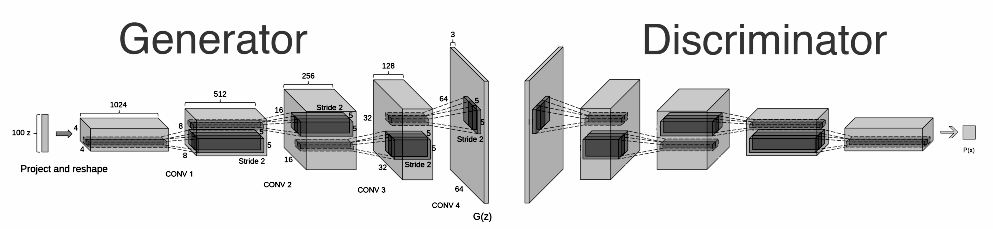
\includegraphics[width=1\textwidth]{images/dcgan.png}
\caption{Deep Convolutional Generative Adversarial Network}
\label{fig:dcgan}
\end{figure}
Today, most GANs are loosely based on the former shown DCGAN \cite{dcgan} architecture. Many papers have focused on improving the setup to enhance stability and performance. Many key insights was given by Salimans \textit{et al}. \cite{improvedgan}, like Usage of convolution with stride instead of pooling, Usage of Virtual Batch Normalization, Usage of Minibatch Discrimination in DD, Replacement of Stochastic Gradient Descent with Adam Optimizer [6], Usage of one-sided label smoothing.
\par\bigskip
% section dcgan (end)
\section{InfoGAN} % (fold)
\label{sec:infogan}
The power of the features encoded in the latent variables was further explored by Chen at al. \cite{infogan}. They propose an algorithm which is completely unsupervised, unlike previous approaches which involved supervision, and learns interpretable and disentangled representations on challenging datasets. Their approach only adds a negligible computation cost on top of GAN and is easy to train.
\par\bigskip

% section infogan (end)

\section{ACGAN} % (fold)
\label{sec:acgan}
Augustus Odena \textit{et al} \cite{acgan} came up a improved training of generative adversarial networks and variant of GAN with employing label conditioning that results in image samples exhibiting global coherence. ACGAN uses an auxiliary classifier to control the minimax game between generator and discriminator. In their work they demonstrate that that adding more structure to the GAN latent space along with a specialized cost function results in higher quality samples
% section acgan (end)

\section{WGAN} % (fold)
\label{sec:wgan}
Another huge development came with the introduction of Wasserstein GANs by Martin Arjovsky \cite{wgan} . He introduced a new algorithm named WGAN, an alternative to traditional GAN training. In this new model, he showed that the stability of learning can be improved, remove problems like mode collapse, and provide good learning curves useful for debugging and hyperparameter searches.
\par\bigskip

This recently proposed Wasserstein GAN (WGAN) \cite{wgan} makes progress toward stable training of GANs, but sometimes can still generate only low-quality images or fail to converge. 
Ishaan Gulrajani with Martin Arjovsky proposed an alternative in \cite{improvedwgan} to fix the issues the previous GAN faced. This proposed method performs better than standard WGAN and enables stable training of a wide variety of GAN architectures with almost no hyperparameter tuning, including 101-layer ResNets \cite{deepresidual} and language models over discrete data.
\par\bigskip

% section wgan (end)
\section{Other GANs} % (fold)
\label{sec:other_gan}
Work by Mehdi Mirza \textit{et al}. \cite{congan} introduced the conditional version of GAN which can be constructed by simply feeding the data, y, we wish to condition on to both the generator and discriminator. The CGAN results were comparable with some other networks, but were outperformed by several other approaches – including non-conditional adversarial nets.
\par\bigskip

Sebastian Nowozin \textit{et al}. \cite{vardivmin} discussed the benefits of various choices of divergence functions on training complexity and the quality of the obtained generative models. They show that any f-divergence can be used for training generative neural samplers. 
\par\bigskip

Ming-Yu \textit{et al}. \cite{copgan} proposed coupled generative adversarial network (CoGAN) for learning a joint distribution of multi-domain images. The existing approaches requires tuples of corresponding images in different domains in the training data set. CoGAN can learn a joint distribution without any tuple of corresponding images.
\par\bigskip

% section other_gan (end)
\section{Capsule Neural Network} % (fold)
\label{sec:capsule_neural_network}
A big breakthrough in the field of Deep Learning came with the introduction of CapsNets or Capsule Networks \cite{capsnet} by the Godfather of Deep Learning, Geoffrey Hinton \textit{et al}. CNNs perform exceptionally great when they are classifying images which are very close to the data set. If the images have rotation, tilt or any other different orientation then CNNs have poor performance. A capsule is a group of neurons whose activity vector represents the instantiation parameters of a specific type of entity such as an object or an object part. They use the length of the activity vector to represent the probability that the entity exists and its orientation to represent the instantiation parameters. Active capsules at one level make predictions, via transformation matrices, for the instantiation parameters of higher-level capsules. When multiple predictions agree, a higher level capsule becomes active. They show that a discrimininatively trained, multi-layer capsule system achieves state-of-the-art performance on MNIST and is considerably better than a convolutional net at recognizing highly overlapping digits. To achieve these results they use an iterative routing-by-agreement mechanism: A lower-level capsule prefers to send its output to higher level capsules whose activity vectors have a big scalar product with the prediction coming from the lower-level capsule.
% section capsule_neural_network (end)
